\chapter{Related Work}
\label{ch:relatedwork}

As a popular entertainment business, music service was always been a popular topic in the industry. Both the recommendation system and music emotions have many existing research projects.

\section{Spotify Recommendation System}

A recommendation system or recommender system is an algorithm that can suggest user-preferred items to a user by giving score or probability to items \cite{ricci2011introduction}. In the music recommendation system, the item to suggest would be music.

Take Spotify as an example, it has three parts in their recommendation system, which are Collaborative Filtering, Natural Language Processing, and Audio Metadata Modeling.

\subsection{Collaborative Filtering}

Collaborative Filtering \cite{Su2009} is an algorithm that recommends new content between similar users or items. The algorithm predicts user preferences by learning from users' past ratings for items  \cite{Celma2010}.

\subsubsection{Item-based}

The first way to do collaborative filtering is to predict the relationship between items. Therefore, calculate item similarity is the first step. The common ways of calculating similarity for item i and j, sim(i,j), are cosine similarity, Pearson correlation, adjusted cosine, and conditional probability.

Let the targeted users be set U, $r_{u, i}$ and $r_{u, j}$ be user's rating over item i and item j. The cosine similarity can be calculated by equation \eqref{eq:1}.

\begin{equation}
  \operatorname{sim}(i, j)=\cos (\mathbf{i}, \mathbf{j})=\frac{\mathbf{i} \cdot \mathbf{j}}{\|i\| *\|j\|}=\frac{\sum_{u \in U} r_{u, i} r_{u, j}}{\sqrt{\sum_{u \in U} r_{u, i}^{2}} \sqrt{\sum_{u \in U} r_{u, j}^{2}}}
  \label{eq:1}
\end{equation}

Let $\bar{r}_{u}$ be the average rating for user $u$. The adjusted cosine can be calculated by equation \eqref{eq:2} \cite{adjustedcosinesimilarity}.

\begin{equation}
  \operatorname{sim}(i, j)=\frac{\sum_{u \in U}\left(r_{u, i}-\bar{r}_{u}\right)\left(r_{u, j}-\bar{r}_{u}\right)}{\sqrt{\sum_{u \in U}\left(r_{u, i}-\bar{r}_{u}\right)^{2}} \sqrt{\sum_{u \in U}\left(r_{u, j}-\bar{r}_{u}\right)^{2}}}
  \label{eq:2}
\end{equation}

Let $\bar{r}_{i}$ be the average rating for item i. The Pearson correlation can be calculated by equation \eqref{eq:3}. One good thing about correlation similarity is that it can calculate how close are the items related \cite{Celma2010}.

\begin{equation}
  \operatorname{sim}(i, j)=\frac{\operatorname{Cov}(i, j)}{\sigma_{i} \sigma_{j}}=\frac{\sum_{u \in U}\left(r_{u, i}-\bar{r}_{i}\right)\left(r_{u, j}-\bar{r}_{j}\right)}{\sqrt{\sum_{u \in U}\left(r_{u, i}-\bar{r}_{i}\right)^{2}} \sqrt{\sum_{u \in U}\left(r_{u, j}-\bar{r}_{j}\right)^{2}}}
  \label{eq:3}
\end{equation}

Finally, the conditional probability can be calculated by equation \eqref{eq:4}.

\begin{equation}
  \operatorname{sim}(i, j)=P(j | i) = \frac{f(i \cap j)}{f(i)}
  \label{eq:4}
\end{equation}

After obtained the similarity between items, a value of the item for the targeted user can be predicted. It means to obtain how the user rates similar items for specific item i, the record we obtained could is the history records.

\subsubsection{User-Based}

Another way to do collaborative filtering is to find the users that are similar. After knowing the similar users, and the item similarity scare are obtained, the recommendations can be predicted.

Take Spotify as an example, after collecting the user interaction, for instance, the playlist, whether liked the song, a unique coordinate will be generated for each user. The collected fields are the dimensions. The item-based suggestion will be coming from analyzing the user playlists, and the user-based suggestion will be coming from comparing different users. Once the similar users are identified, the algorithm will simply recommend contents that one user has and others do not.

\subsection{Natural Language Processing}

Natural language processing is the study of the interaction between computers and human languages. Human language can be speeches or writings. This study has many sub-fields, for example, speech recognition, text summarization, and text generation. By using natural language processing techniques, the meaning of lyrics can be classified, which can be further used to identify the music genre. The sentiment of the lyrics can also be analyzed, which can be used to identify the mood of the music tracks.

\subsubsection{Text Sentiment Classification}

Text classification is a very important sub-field of natural language processing, many real-life applications are depending on text classification. For example, web search, document classification, and information ranking \cite{joulin2016bag}. The classification can be based on different aspects, in music recommendation examples, sentiment can be a feature. Sentiment analysis is the contextual mining of text emotions, for instance, positive or negative. Happiness, joyful, and compliment emotions can be categorized as positive emotions. Sad, angry, and guilt can be categorized as negative emotions. The general text classification workflow is shown in figure \ref{tcworkflow}.

\begin{figure}[htbp]
\centering
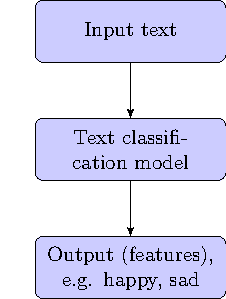
\includegraphics[width=2.5 in]{images/tcworkflow}
\caption{Text Classification Workflow}
\label{tcworkflow}
\end{figure}

The first step to classify text is to treat text as a bag of words \cite{Brilis2012}. Bag of words is a model in natural language processing that treats texts as unordered words, and the frequency of each word would be recorded. This process is usually conducted by tokenization, and followed by stemming and lemmatization. Stemming and lemmatization can delete the additional part of the word, remain only the stem part. For example, after stemming and lemmatization, the word "interesting" would become "interest". After stemming and lemmatization, stop words, which are words that have no actual meaning in a sentence, will be removed from the bag of words. An example of a stop word can be "and".

One way to classify texts is a Naive Bayes algorithm. Naive Bayes is based on Bayes’ probability theorem \cite{DBLP:journals/corr/Raschka14}. In Bayes’ probability theorem, for event A and B, the conditional probability of A given B is equation \eqref{eq:5}.

\begin{equation}
  P(A | B)=\frac{P(B | A) \cdot P(A)}{P(B)}
  \label{eq:5}
\end{equation}

Multinomial naive Bayes is one of the ways to use the Naive Bayes algorithm to classify texts. It uses the term frequency, $tf(t,d)$, where $t$ is term, and $d$ is the active document. Let $tf(t,d)$ be the frequency of term $t$ in document $d$, and $n_{d}$ be the total number of terms in document. As the equation \eqref{eq:6} shows.

\begin{equation}
  \text { term frequency }=\frac{t f(t, d)}{n_{d}}
  \label{eq:6}
\end{equation}

Spotify uses textual information from the internet to find key terms for music content. The terms will be used to build vectors for each song. A similar technique used in collaborative filtering will be applied to find similar content. This technique has a flaw that the textual information gets from the internet is too broad. It will be better if the information is from the comments under each song directly. That way, each song will have a direct correlation to the key terms. Except for comments, user search history could also be used as part of the text \cite{Bu2010}.

\subsection{Audio Metadata Modeling}

Audio metadata is the information for the audio files, it usually contains names for artist, album, title, genre, track number, and more \cite{audio2018}. After sampling the audio, more information can be included in audio metadata, for example, loudness, tempo, and more. This information can be used to predict potential music or human emotions. Tempo represents the speed of the audio, it is related to human emotions according to studies. Fast tempo and emotions like joy and fear have correlations, slow tempo and emotions like sadness and tenderness have correlations \cite{kamenetsky1997effect}.

Spotify has a database that contains the audio metadata. These aspects can be used to build vector representations. By applying a similar technique in collaborative filtering, similar content will be identified. Bogdanov et al. proposed a way of classifying music by using audio metadata \cite{bogdanov2013semantic}. They asked participants to choose their preferred music and categorized them based on their preferences. They then modeled the audio files and classified them. After that, they correlated the classified features with predefined categories. By using this model, they can suggest songs based on audio metadata.

\section{Content-Based Music Information Retrieval}

Besides collaborative filtering, content-based music information retrieval is another effective way of recommending. This method collects information that describes the music, and use the information to suggest new content. Audio metadata can be one of the sources for the information.

One application is to collect and classify audio signal features, then apply them to match based on different situations. In general, there are two ways of matching, which are query by example, and query by humming \cite{Kaminskas2012}. Query by example means getting the audio signal as input and return music metadata as output. This query method works on the specific music track, but not the variation tracks, for example, a cover version. Query by humming makes it up by getting melody as input and returns similar tracks. This application is more of a searching or matching algorithm. The limitation of this recommendation method is as I mentioned previously, lack of novelty \cite{Kaminskas2012}. It only expands on user saved songs, and it cannot predict user situation.

The other application is to combine the information which describes the music with user preferences. The user preference does not mean the user ratings, content-based music recommendation does not rely on user ratings \cite{Celma2010}. However, categorizing music content based on descriptive information requires experts of the fields to set rules. A similarity check is also required for the content-based suggestion. The way of calculating the similarity between two items is through calculating their distance. The common ways of calculating such distance are Euclidean distance \eqref{eq:7}, Manhattan distance \eqref{eq:8}, vector cosine distance\eqref{eq:1}, Mahalanobis distance \eqref{eq:9}, and Chebyshev distance \eqref{eq:10}.

\begin{equation}
  d=|x-y|=\sqrt{\sum_{i=1}^{n}\left|x_{i}-y_{i}\right|^{2}}
  \label{eq:7}
\end{equation}

Euclidean distance measures the straight line between two points in N-dimensional space \cite{euclidean}.

\begin{equation}
  d(x, y)=\sum_{i=1}^{n}\left|x_{i}-y_{i}\right|
  \label{eq:8}
\end{equation}

Manhattan distance is also a measurement of the straight line between two points in N-dimensional space. Just imagine the street blocks in Manhattan, there two paths from one intersection to the other one. However, the true distance between them is a straight line cut through the buildings \cite{craw1970}.

\begin{equation}
  d(x, y)=\sqrt{(x-y)^{T} S^{-1}(x-y)}
  \label{eq:9}
\end{equation}

Mahalanobis distance is a measurement of the straight line distance between two points in N-dimensional space. Mahalanobis distance handles better with correlated points($\ge2$). In situations that there are more than 2 points that are correlated, the axes of the points are no longer orthogonal, and they cannot be plotted in 3-dimensional space \cite{stephanie2018}.

\begin{equation}
  d(x, y)=\max _{i=1 . . . n}\left|x_{i}-y_{i}\right|
  \label{eq:10}
\end{equation}

Chebyshev distance, also called maximum value distance, is similar to Euclidean distance and Manhattan distance. It calculates the straight line distance based on point coordinates.

There are limitations for this application when new users entered the system, they can't get the right suggestion because the system needs time to adjust to the user preferences. This situation is also called the cold-start problem \cite{Celma2010}. Another issue is feature extraction. It is hard to extract high-level descriptions such as mood. These high-level descriptions are very important in accurate and personalized recommendations.

\section{Contextual Music Retrieval}

Contextual music information is any information, other than music content information, that describes the music content itself. Contextual music suggestion means to recommend music based on the user's actual situation, for example, emotional state. This method takes three sources of information, environment-related context, user-related context, and multimedia context \cite{Kaminskas2012}. Environment-related information can be the season, temperature, time, and weather because all these contexts can influence human emotions. User-related information can be user activities, such as exercising and driving, user profiles, such as social network statements, and emotional state. Multimedia can be text and image relevant to the music. This information can be used to profile and predict the user's actual situation. After the necessary information is gathered, similarity predicts, classification, and other techniques can be used to predict user preferences.

Another way of achieving contextual music retrieval is proposed by B. Han et al \cite{Han2010}. They proposed an emotion state transition model which models music-evoked human emotions, and content-based music recommendation ontology to profile user preference and context. The system provides music by mapping high-dimensional music features with the emotion state transition model. According to the paper, this method achieved 67.54\% overall accuracy. The limitation of this method is that it needs a large amount of data, and the human emotional state can be changed based on the social environment. Once the social context is changed, more data would be required to get higher accuracy.

Recommendation based on contextual music retrieval is still new, and it has great potential to contribute to the music recommendation system.
